\documentclass{beamer}

\usepackage{beamerthemeshadow}
\usepackage{color}
\usepackage{verbatim}
\usepackage{tikz}
\usetikzlibrary{shapes,arrows,positioning,calc}
\usepackage[normalem]{ulem}
\usepackage[timeinterval=10]{tdclock}
%\usepackage{wrapfig}

\mode<presentation>
{
 \usetheme{Warsaw} %%% Change later
\usecolortheme{dove}

%gets rid of bottom navigation bars
%\setbeamertemplate{footline}[page number]{}

% a version with clock in the footline
\setbeamertemplate{footline}
{%
\begin{beamercolorbox}[wd=1.0\paperwidth,ht=2.25ex,dp=1ex,right]{date in head/foot}%
           \usebeamerfont{date in head/foot} \msdark{\insertshortdate{\tdtime}\hspace*{2em}
           \insertframenumber{} / \inserttotalframenumber\hspace*{2ex}} 
        \end{beamercolorbox}%
}

  \setbeamercovered{transparent}
  % or whatever (possibly just delete it)
}


\usepackage{graphicx}

\usepackage{amssymb,soul}

\usepackage{hyperref}

\definecolor{myblue}{rgb}{0, 0, 0.9}

\definecolor{mygreen}{rgb}{0,0.6,0}

\definecolor{mymagenta}{rgb}{0.9, 0, 0.9}

\definecolor{myred}{rgb}{0.9,0,0}

\definecolor{mygray}{rgb}{0.8,0.8,0.8}

\definecolor{mydark}{rgb}{0.4, 0.4, 0.4}

\definecolor{myblack}{rgb}{0,0,0}

\newcommand{\msblue}[1]{{\color{myblue} #1}}

\newcommand{\msmagenta}[1]{{\color{mymagenta} #1}}

\newcommand{\msred}[1]{{\color{myred} #1}}

\newcommand{\msgreen}[1]{{\color{mygreen} #1}}

\newcommand{\msgray}[1]{{\color{mygray} #1}}

\newcommand{\msdark}[1]{{\color{mydark} #1}}

\newcommand{\msblack}[1]{{\color{myblack} #1}}

\newcommand{\relu}{\mbox{\bf ReLU}}

\begin{document}

\title{Let's think about embedding neural machines into modulating fields}
\author{\msmagenta{\bf Mishka (Michael Bukatin)}}
\institute[DMM] % (optional, but mostly needed)
{\href{https://github.com/anhinga}{\tt\small github:anhinga}\\
\ \\
{\small Dataflow Matrix Machines project}
}
\date[]  
{
Longevity, AI, and Cognitive Research Hackathon\\
Cambridge, MA, October 27, 2024}

\begin{frame}
%  \initclock
  \titlepage
\end{frame}

\section{Biological vs artificial}


\begin{frame}

  \frametitle{Case for the role of electromagnetic fields in neuro}

\begin{itemize}

\item {\bf Michael Levin:}

\begin{itemize}

\item {\bf Strong case: electromagnetic fields are crucial in\\ biological computations}

\end{itemize}

\ \\

\item Andrés Gómez-Emilsson and others: 

\begin{itemize}

\item Conjecture: qualia fields are carried by electromagnetic fields

\end{itemize}

\ \\

\item  Joscha Bach and others:

\begin{itemize}

\item Conjecture: bodies are antennas (receive and transmit)

\end{itemize}

\ \\

\item  This all fits together, would explain a lot

\end{itemize}

\end{frame}

\begin{frame}

  \frametitle{Two routes}

\ \\

\begin{itemize}

\item Biorealistic

\begin{itemize}

\item Realistic neural nets and electromagnetic fields

\item Even understanding how {\it C elegans} works would be nice

\item Very important, quite difficult 

\end{itemize}


\ \\

\item Artificial architectures and ``artificial fields"

\begin{itemize}

\item Inspired by how we do ``artificial attention"

\item Small-scale efforts have good chances for progress

\item {\bf Needs a guiding light (what are we looking for?)}

\end{itemize}

\end{itemize}

\end{frame}

\begin{frame}

\frametitle{Biological attention vs ``artificial attention"}

\begin{itemize}

\item Biological attention

\begin{itemize}

\item Synchronized oscillations ({\it some} of the gamma waves)

\item Crick-Koch ``40hz conjecture"  (30hz-70hz)

\begin{itemize}
\item ``Towards a neurobiological theory of consciousness" (1990)
\end{itemize}

\end{itemize}


\ \\

\item ``Artificial attention"

\begin{itemize}

\item Linear combinations of ``feature vectors"

\item Forget about the biological mechanism; \msmagenta{just model the effects}

\begin{itemize}
\item Some features are emphasized, others are suppressed
\end{itemize}

\item Surprisingly effective, especially in hierarchies (Transformers)

\end{itemize}

\end{itemize}

\end{frame}

\begin{frame}

\frametitle{``Artificial modulation": what should be the guiding light?}

{\bf What should be the guiding light for modulation of\\ artificial neural machines by
artificial fields?}\\[2ex]

Effectiveness in various tasks\\ (better training, better fine-tuning, better inference).\\[2ex]

The artificial fields can be

\begin{itemize}
\item induced by neural machines themselves
\item external
\item a mix of both\\[2ex]
\end{itemize}

One can modulate network inputs, network outputs,\\ network connectivity weights,
and other parameters\\ (e.g. parameters of ``activation functions")

\end{frame}

\begin{frame}

\frametitle{This has been the new part for this hackaton}

Now I am going to tell you something which has been known before which is likely to be helpful
if one wants to attack this problem.

\end{frame}

\section{Dataflow matrix machines (DMMs)}

\begin{frame}

\frametitle{What's the full generality here?}

The essence of neural model of computations is that\\
\msmagenta{linear and non-linear computations are interleaved.}\\[2ex] 

What is the most general (and most flexible) way\\
to make this linear/non-linear alternating pattern possible?\\[2ex]

\dotfill\\[2ex]

The natural degree of generality for neural-like computations is:\\[2ex]
\hspace{0.2in}\sout{use only streams of numbers}\\
\hspace{0.2in}use any streams supporting the notion of\\
\hspace{0.6in}linear combination of several streams \msmagenta{(``linear streams")}

\end{frame}

\begin{frame}

  \frametitle{\msmagenta{Dataflow matrix machines (DMMs)}}

DMMs: a very natural class of {\bf neural machines}.\\[2ex]

They use arbitrary {\bf linear streams} instead of streams of numbers.\\[2ex]

{\bf Use of linear streams by single neurons} is the main source of their power compared to RNNs.
The extra power also comes from:\\[1ex]

\begin{itemize}

\item Arbitrary fixed or variable arity of neurons;\\[2ex]

\item Highly expressive linear streams of V-values\\ (tree-shaped flexible tensors);\\[2ex]

\item Unbounded network size ($\Rightarrow$ unbounded memory);\\[2ex]

\item Self-referential facilities: ability to change weights, topology, and the size of the active part dynamically, on the fly.

\end{itemize}

\end{frame}

\subsection{Linear streams}

\begin{frame}

  \frametitle{\msmagenta{RNNs: linear and non-linear computations are interleaved}}



\begin{columns}[T]
\begin{column}{0.5\textwidth}
\begin{tikzpicture}
   \clip (-2.0, -2.0) rectangle (4.0, 2.0);
   %\draw (-2.0, -2.0) rectangle (4.0, 2.0);
   \draw [->] (-0.8, 0) -- (-0.8, 1) node [left] {$i_m$};
   \draw [->] (-1.6, 0) -- (-1.6, 1) node [left] {$i_1$};
   \filldraw (-1.2,0) circle [radius=0.5pt]
                 (-1.4,0)  circle [radius=0.5pt]
                 (-1.0, 0) circle [radius=0.5pt]
                 (-0.8, 0) circle [radius=1pt]
                 (-1.6, 0) circle [radius=1pt];

 

 \msgreen{  \draw [->] (-0.4, -1) node [left] {\msblack{$x_1$}} -- (-0.4, 1) node [midway, above right] {$f_1$} node [right] {\msblack{$y_1$}};
   \draw [->] (0.4, -1)  node [left] {\msblack{$x_k$}} -- (0.4, 1) node [midway, above right] {$f_k$} node [right] {\msblack{$y_k$}};}
   \filldraw (0,0) circle [radius=0.5pt]
                 (-0.2,0)  circle [radius=0.5pt]
                 (0.2, 0) circle [radius=0.5pt];

   \draw (0.8, -1) node [right] {$o_1$} -- (0.8, 0);
   \draw (1.6, -1) node [right] {$o_n$} -- (1.6, 0);
   \filldraw (1.2,0) circle [radius=0.5pt]
                 (1.4,0)  circle [radius=0.5pt]
                 (1.0, 0) circle [radius=0.5pt]
                 (0.8, 0) circle [radius=1pt]
                 (1.6, 0) circle [radius=1pt]; 

\msblue{\draw [->, very thick] (0, 1.2) .. controls (3.5, 4.2) and (3.5, -4.2) .. (0, -1.2)  node [midway, right] {{\bf W}};}

\end{tikzpicture}

\end{column}
\begin{column}{0.5\textwidth}

``Two-stroke engine" for an RNN:\\[3ex]


``Down movement" \msblue{(linear$^1$)}:\\[2ex] 

$(x_1^{t+1}, \ldots, x_k^{t+1}, o_1^{t+1}, \ldots, o_n^{t+1})^{\top}=$\\[0.1ex] \msblue{{\bf W}}$ \cdot (y_1^{t}, \ldots, y_k^{t}, i_1^{t}, \ldots, i_m^{t})^{\top}$.\\[3ex]

``Up movement" \msgreen{(non-linear$^2$)}:\\[2ex]  

$y_1^{t+1} = \msgreen{f_1}(x_1^{t+1}), \ldots,$\\[0.1ex]$y_k^{t+1} = \msgreen{f_k}(x_k^{t+1})$.

\end{column}
\end{columns}

\hrulefill

\msblue{\footnotesize $^1$ linear and global in terms of connectivity}\\
\msgreen{\footnotesize $^2$ usually non-linear, local}

\end{frame}


\begin{frame}

\frametitle{\msmagenta{Linear streams}}

The key feature of {\bf DMMs} compared to {\bf RNNs}:
         they use\\ {\bf linear streams} instead of streams of numbers.\\[2ex]

The following streams all support the pattern of alternating\\ linear and non-linear computations:\\[2ex]

\begin{itemize}

\item Streams of numbers\\[2ex]

\item Streams of vectors from fixed vector space $V$\\[2ex]

\item Linear streams: such streams that the notion of\\ {\bf linear combination of several streams} is defined.\\[3ex]

\end{itemize}

\msmagenta{{\bf ``Artificial attention"}:\\ taking linear combinations of high-dimensional objects.}






\end{frame}




\begin{frame}

\frametitle{Kinds of linear streams}

\msmagenta{The notion of {\bf linear streams} is more general than the notion
of {\bf streams of vectors}.} Some examples:\\[1ex]


\begin{itemize}


\item Every vector space $V$ gives rise to the corresponding kind of linear streams
(streams of vectors from that space)\\[2ex]

\item \msmagenta{Every measurable space $X$ gives rise to the space of\\ {\bf streams of
probabilistic samples} drawn from $X$\\ and decorated with +/- signs\\
(linear combination is defined by a stochastic procedure)}\\[2ex]

\item Streams of images of a particular size (that is, animations)\\[2ex]

\item Streams of matrices; streams of multidimensional arrays\\[2ex]

\item Streams of V-values based on nested maps (\msmagenta{trees})\\[2ex]



\end{itemize}

\end{frame}








\begin{frame}

  \frametitle{\msmagenta{Dataflow matrix machines  (DMMs, continued)}}

Countable network with finite active part at any moment of time.\\[2ex]

Countable matrix \msblue{{\bf W}} with finite number of non-zero elements at any moment of time.

\begin{columns}[T]
\begin{column}{0.7\textwidth}
\begin{tikzpicture}
   \clip (-3.0, -2.0) rectangle (5.0, 2.0);
   %\draw (-2.0, -2.0) rectangle (4.0, 2.0);
  \filldraw (-3.2,0) circle [radius=0.5pt]
                (-3.0,0)  circle [radius=0.5pt]
                (-3.4, 0) circle [radius=0.5pt]; 

\msgreen{   \draw [->] (-1.2, 0) -- (-0.8, 1) node [right] {\msblack{$y_{2,C_1}$}};
   \draw [->] (-1.2, 0) -- (-1.6, 1) node [left] {\msblack{$y_{1,C_1}$}};
   \draw (-2.0, -1)  node [left] {\msblack{$x_{1,C_1}$}} -- (-1.2, 0);
   \draw (-1.2, -1)  node [below] {\msblack{$x_{2,C_1}$}} -- (-1.2, 0) node [left] {$f_{C_1}$};
   \draw (-0.4, -1)  node [right] {\msblack{$x_{3,C_1}$}} -- (-1.2, 0);}


  \filldraw (0,0) circle [radius=0.5pt]
                (-0.2,0)  circle [radius=0.5pt]
                (0.2, 0) circle [radius=0.5pt];


 \msgreen{    \draw (1.6, -1) node [left] {\msblack{$x_{1,C_2}$}} -- (2.0, 0)  node [left] {$f_{C_2}$};;
   \draw (2.4, -1) node [right] {\msblack{$x_{2,C_2}$}} -- (2.0, 0);
   \draw [->] (2.0, 0) -- (1.2, 1) node [left] {\msblack{$y_{1,C_2}$}};
   \draw [->] (2.0, 0) -- (2.0, 1) node [above] {\msblack{$y_{2,C_2}$}};
   \draw [->] (2.0, 0) -- (2.8, 1) node [right] {\msblack{$y_{3,C_2}$}};}


  \filldraw (3.2,0) circle [radius=0.5pt]
                (3.0,0)  circle [radius=0.5pt]
                (3.4, 0) circle [radius=0.5pt]; 


  \msblue{\draw [->, very thick] (0.5, 1.2) .. controls (5.5, 4.2) and (5.5, -4.2) .. (0.5, -1.2)  node [midway, right] {{\bf W}};}

\end{tikzpicture}

\end{column}
\begin{column}{0.3\textwidth}

{%\scriptsize
\tiny
``Down movement": 

\msblue{For all inputs $x_{i,C_k}$ where there is a non-zero weight $w_{(i,C_k), (j,C_m)}^t$:}\\[1ex]

{\scriptsize$x_{i,C_k}^{t+1} = \msblue{\sum}_{\{(j,C_m) | w_{(i,C_k), (j,C_m)}^t \neq 0\}}$\\[0.1ex]$\msblue{w_{(i,C_k), (j,C_m)}^t }* y_{j, C_m}^{t}.$}\\[3ex]

``Up movement":\\[0.1ex]  

\msgreen{For all active neurons $C$:}\\[1ex]

{\scriptsize $y^{t+1}_{1,C},...,y^{t+1}_{p,C} = \msgreen{f_C} (x^{t+1}_{1,C},...,x^{t+1}_{n,C})$.}
}

\end{column}
\end{columns}


Here $x_{i,C_k}$ and $y_{j,C_m}$ are linear streams.\\
\msmagenta{Neurons in DMMs have arbitrary arity!}

\end{frame}


\begin{frame}

\frametitle{Skip to slide 27}

The slides 14-26 are here just for convenience\\ if one wants to ponder this further later.

\end{frame}




\section{V-values and variadic neurons}







\begin{frame}

  \frametitle{Type correctness condition  for mixing different kinds of linear streams in one DMM}


\msmagenta{Type correctness condition:} $w_{(i,C_k), (j,C_m)}^t$ is allowed to be
non-zero only if $x_{i,C_k}$ and $y_{j, C_m}$ belong to the same {\bf kind} of linear streams.\\[6ex]

{\bf Next:} \msmagenta{linear streams of {\bf V-values} based on {\bf nested dictionaries}:}\\[2ex]

\begin{itemize}

\item sufficiently universal and expressive to save us from the need to impose type correctness conditions.\\[2ex]

\item allow us to define {\bf variadic neurons}, so that we don't need to keep track of input and output
arity either.
\end{itemize}

\end{frame}








\subsection{Vectors based on nested maps}


\begin{frame}

  \frametitle{\msmagenta{V-values: vector space based on nested dictionaries}}


V-values play the role of Lisp S-expressions in this formalism.\\[3ex]


We want a vector space.\\[3ex]

Take prefix trees with numerical leaves\\ implemented as nested dictionaries.\\[3ex]

We call them {\bf V-values}
(``vector-like values").\\[3ex]

\hrulefill

(A more general construction of V-values with ``linear stream" leaves:  Section 5.3 of \href{https://arxiv.org/abs/1712.07447}{\tt\footnotesize  https://arxiv.org/abs/1712.07447})

\end{frame}





\begin{frame}

  \frametitle{\msmagenta{Ways to understand V-values}}

Consider ordinary words (``labels") to be letters of a countable ``super-alphabet" $L$.\\[2ex]

V-values can be understood as

\begin{itemize}

  \item Finite linear combinations of finite strings of letters from $L$;
  \item Finite prefix trees with numerical leaves;
  \item Sparse ``tensors of mixed rank" with finite number of non-zero elements;
  \item Recurrent maps (that is, nested dictionaries) from $V \cong \mathbb{R}\oplus (L \rightarrow V)$  admitting finite descriptions.

\end{itemize}

\end{frame}


\begin{frame}

  \frametitle{\msmagenta{Example of a V-value: different ways to view it}}

\begin{columns}[T]
\begin{column}{0.5\textwidth}

\begin{tikzpicture}
  \clip (-3.0, -4.5) rectangle (3.0, 0.0);

  \draw[->](0, 0) -- (-1.8, -1)  node [below] {3.5};

  \draw[->](0, 0) -- (0, -1) node [midway,  below right] {:foo};

    \draw[->](0, -1) -- (0.5, -2) node[midway, below right] {\ :bar};

      \draw[->](0.5, -2) -- (0.5, -3) node [below] {7};

    \draw[->](0, -1) -- (-0.5, -2) node [below] {2};

  \draw[->](0, 0) -- (1.8, -1) node [midway, below  right] {\ \ \ \ \ \ :baz};

      \draw[->](1.8, -1) -- (1.8, -2) node [midway, below  right] {:foo};

      \draw[->](1.8, -2) -- (1.8, -3) node [midway, below  right] {:bar};      

      \draw[->](1.8, -3) -- (1.8, -4) node [below] {-4};
 

  \filldraw (1.8, -1) circle [radius=0.7pt]
                (1.8, -2) circle [radius=0.7pt]
                (1.8, -3) circle [radius=0.7pt]
                (0, -1) circle [radius=0.7pt]
                (0.5, -2) circle [radius=0.7pt];
  
 

\end{tikzpicture}
\end{column}
\begin{column}{0.5\textwidth}

\begin{itemize}

{\footnotesize

 \item 3.5 $\cdot$ ($\epsilon$) + 2 $\cdot$ (:foo) + \\ 7 $\cdot$ (:foo :bar) - 4 $\cdot$ (:baz :foo :bar)

 \item ($\leadsto$ 3.5) + (:foo $\leadsto$  2) +\\ (:foo $\leadsto$ :bar $\leadsto$ 7) +\\
          (:baz $\leadsto$ :foo $\leadsto$ :bar $\leadsto$ -4)


\msmagenta{
 \item {\tiny  scalar 3.5 + sparse 1D array \{{\tt d1[:foo]= 2}\} +\\[1.5ex] sparse 2D
matrix \{{\tt d2[:foo, :bar]= 7}\} +\\  sparse 3D array \{{\tt d3[:baz, :foo, :bar]= -4}\}}
}

 \item {\tt \{:number 3.5,\\ :foo \{:number 2, :bar 7\}, :baz \{:foo \{:bar -4\}\}\}}
          ({\tt :number} $\not\in L$)

}

\end{itemize}

\end{column}
\end{columns}

\end{frame}






\subsection{Variable arity}


\begin{frame}

  \frametitle{Dataflow matrix machines (DMMs) based on\\
 streams of  V-values
 and
 variadic neurons}

$x_{f, n_f, i}^{t+1} = \sum_{g \in F} \sum_{n_g \in L} \sum_{o \in L} \msblue{w_{f, n_f, i;\, g, n_g, o}^t} * y_{g, n_g, o}^t$ {\small \msblue{(down movement)}}\\[2ex]

$y_{f, n_f}^{t+1} = f(x_{f, n_f}^{t+1})$ {\small \msgreen{(up movement)}}

\begin{tikzpicture}
  %\draw (-3.5, -2.0) rectangle (7.0, 2.0);
  \clip (-3.5, -2.0) rectangle (7.0, 2.0);

  \filldraw (-3.2,0) circle [radius=0.5pt]
                (-3.0,0)  circle [radius=0.5pt]
                (-3.4, 0) circle [radius=0.5pt]; 

\msgreen{\draw [->] (-2.6, -1.5) node[right] {\msmagenta{$x_{f, n_f}$}} -- (-2.6, 1.5) node [midway, above right] {$f$} node[right] {\msmagenta{$y_{f, n_f}$}};}

  \filldraw (0,0) circle [radius=0.5pt]
                (-0.2,0)  circle [radius=0.5pt]
                (0.2, 0) circle [radius=0.5pt];

\msgreen{\draw [->] (0.6, -1.5) node[right] {\msmagenta{$x_{g, n_g}$}} -- (0.6, 1.5) node [midway, above right] {$g$} node[right] {\msmagenta{$y_{g, n_g}$}};}

  \filldraw (3.2,0) circle [radius=0.5pt]
                (3.0,0)  circle [radius=0.5pt]
                (3.4, 0) circle [radius=0.5pt]; 


 \msblue{ \draw [->, very thick] (1.1, 1.1) .. controls (5.5, 4.3) and (5.5, -4.0) .. (1.1, -0.8)  node [midway, right] {{\bf W}};}

  \foreach \y in {-1.0, 1.0}
    {

      \draw [densely dotted] (0.45, \y+0.15) ellipse [x radius=100pt, y radius=4pt];

     \foreach \x in {-1.0, 2.2}
       {

        \foreach \d in {-0.4, -0.15, 0.1}
           {
               \msmagenta{\draw(\x-0.15, \y + 0.45) -- (\x+\d, \y+0.15); 
               \draw (\x+\d, \y + 0.15) -- (\x+\d-0.08, \y-0.15);
               \draw (\x+\d, \y + 0.15) -- (\x+\d+0.08, \y-0.15);
               \filldraw (\x+0.5*\d-0.05, \y-0.25) circle [radius=0.2pt];
               \filldraw (\x+0.5*\d+0.5, \y+0.15) circle [radius=0.2pt];}
           }
       } 
     }
 
\end{tikzpicture}

\end{frame}

\section{Programming patterns and self-referential facilities}




\begin{frame}

  \frametitle{\msmagenta{DMMs: programming with powerful neurons}}

Powerful variadic neurons and streams of V-values $\Rightarrow$ a much more expressive formalism
 than networks based on streams of numbers.\\[2ex]

$\Rightarrow$ Many tasks can be accomplished by \msmagenta{compact DMM networks},\\
 where {\bf single neurons function as layers or modules}.

\hrulefill

\begin{itemize}

\item \msmagenta{Accumulators and memory}

\item Multiplicative constructions and ``fuzzy if"

\item \msmagenta{Sparse vectors}

\item Data structures

\item Self-referential facilities

\end{itemize}






\end{frame}

\begin{frame}

  \frametitle{\msmagenta{Accumulators and memory}}

\begin{tikzpicture}
   \clip (-2.0, -2.0) rectangle (7.0, 2.0);




  \filldraw (0,0) circle [radius=0.5pt]
                (-0.2,0)  circle [radius=0.5pt]
                (0.2, 0) circle [radius=0.5pt];

\msgreen{\draw [->] (0.6, -1.5) node[right] {\msblack{$x_{{\tt plus}, {\tt :my\mbox{\footnotesize -}neuron}}$}} -- 
                    (0.6, 1.5) node [midway, above right] {\tt plus} node[right]
                    {\msblack{$y_{{\tt plus}, {\tt :my\mbox{\footnotesize -}neuron}}$}};}

  \filldraw (3.2,0) circle [radius=0.5pt]
                (3.0,0)  circle [radius=0.5pt]
                (3.4, 0) circle [radius=0.5pt]; 


 \msblue{\draw [->] (1.9, 1.1) .. controls (5.5, 4.3) and (5.5, -4.0) .. (2.15, -0.85)  node [midway, left] {{1.0}};

  \draw [->] (1.7, -0.2) -- (1.5, -0.9);
  \filldraw (1.5, -0.25) circle [radius=0.2pt];
  \filldraw (1.6, -0.25) circle [radius=0.2pt];
  \filldraw (1.4, -0.25) circle [radius=0.2pt];
  \draw [->] (1.3, -0.2) node [left] {{\tiny updates from other neurons}} -- (1.5, -0.8);}


  \foreach \y in {-1.0}
    {

      \draw [densely dotted] (1.0, \y+0.15) ellipse [x radius=80pt, y radius=5pt];

     \foreach \x in {2.0}
       {

        \foreach \d in {-0.4}
           {
               \draw(\x-0.15, \y + 0.45) -- (\x+\d, \y+0.15) node [left] {\scriptsize{\tt :delta}}; 
               \draw (\x+\d, \y + 0.15) -- (\x+\d-0.08, \y-0.15);
               \draw (\x+\d, \y + 0.15) -- (\x+\d+0.08, \y-0.15);
               \filldraw (\x+0.5*\d-0.05, \y-0.25) circle [radius=0.2pt];
               %\filldraw (\x+0.5*\d+0.5, \y+0.15) circle [radius=0.2pt];
           }
       \foreach \d in {0.1}
           {
               \draw(\x-0.15, \y + 0.45) -- (\x+\d, \y+0.15) node [right] {\scriptsize{\tt :accum}}; 
               \draw (\x+\d, \y + 0.15) -- (\x+\d-0.08, \y-0.15);
               \draw (\x+\d, \y + 0.15) -- (\x+\d+0.08, \y-0.15);
               \filldraw (\x+0.5*\d-0.05, \y-0.25) circle [radius=0.2pt];
               %\filldraw (\x+0.5*\d+0.5, \y+0.15) circle [radius=0.2pt];
           }
        \foreach \d in {-0.4, -0.15, 0.1}
           {
              \filldraw (\x+0.5*\d-0.05, \y-0.25) circle [radius=0.2pt];
           }
       } 
     }

  \foreach \y in {0.9}
    {

      \draw [densely dotted] (1.0, \y+0.15) ellipse [x radius=80pt, y radius=5pt];

     \foreach \x in {2.0}
       {

        \foreach \d in {-0.15}
           {
               \draw(\x-0.15, \y + 0.45) -- (\x+\d, \y+0.15) node [right] {\scriptsize{\tt :single}}; 
               \draw (\x+\d, \y + 0.15) -- (\x+\d-0.08, \y-0.15);
               \draw (\x+\d, \y + 0.15) -- (\x+\d+0.08, \y-0.15);
 
               %\filldraw (\x+0.5*\d+0.5, \y+0.15) circle [radius=0.2pt];
           }
        \foreach \d in {-0.4, -0.15, 0.1}
           {
              \filldraw (\x+0.5*\d-0.05, \y-0.25) circle [radius=0.2pt];
           }
       } 
     }
 
\end{tikzpicture}

In this implementation, activation function \msgreen{\footnotesize \tt plus} adds V-values from 
{\footnotesize\tt :accum} and {\footnotesize\tt :delta}
together and places the result into {\footnotesize\tt :single}.

\end{frame}

\begin{frame}

  \frametitle{Multiplicative masks and fuzzy conditionals (gating)}

\msmagenta{Many multiplicative constructions enabled by {\bf input arity $>1$}.}\\[2ex]

The most notable is multiplication of an otherwise computed
neuron output by the value of one of its scalar inputs.\\[2ex]

This is essentially a {\bf fuzzy conditional}, which can
\begin{itemize} 
\item selectively
turn parts of the network on and off in real time\\ via multiplication by zero
\item attenuate or amplify the signal
\item  reverse the signal
via multiplication by -1
\item  redirect
flow of signals in the network
\item ... \\[2ex]
\end{itemize}

\end{frame}


\subsection{Sparse vectors}



\begin{frame}

  \frametitle{\msmagenta{Sparse vectors of high or infinite dimension}}

Example:  a neuron accumulating count of words in a given text.\\[2ex]

The dictionary mapping words to their respective counts is an infinite-dimensional vector
with a finite number of non-zero elements.\\[2ex]

\msmagenta{\Large $\bullet$} Don't need a neuron for each coordinate of our vector space.\\[2ex]

 \msmagenta{\Large $\bullet$} Don't have an obligation to reduce dimension by embedding.

\end{frame}





\subsection{Data structures}





\begin{frame}

  \frametitle{Streams of immutable \msmagenta{data structures}}

One can represent {\bf lists, matrices, graphs,} and so on\\ via nested dictionaries.\\[3ex]


It is natural to use streams of immutable V-values in the implementations of DMMs.\\[3ex]

The DMM architecture is friendly towards algorithms working with immutable data structures in
the spirit of functional programming.\\[3ex]

But more imperative styles can be accommodated as well.

\end{frame}





\subsection{Self-referential facilities}

\begin{frame}

  \frametitle{\msmagenta{Self-referential facilities}}

Difficult to do well with streams of scalars because of dimension mismatch:
typically one has $\sim N$ neurons and $\sim N^2$ weights.\\[2ex]

\msmagenta{Easy in DMMs:}\\[2ex]

It is easy to represent the network matrix {\bf W} as a V-value.\\[2ex]

Emit the stream
of network matrices from neuron {\tt Self}.\\[2ex]

Use the most recent V-value from that stream
as the network matrix {\bf W} during the
next ``down movement".\\[2ex]

This mechanism allows a DMM network to 
{\bf modify its own weights, topology, and size}
while it is running.

\end{frame}


\begin{frame}

  \frametitle{\msmagenta{Self-referential facilities}}

Our current implementation: {\tt Self} connected as an accumulator.\\[2ex]
It accumulates the value of the network matrix and
accepts additive updates from other neurons in the network.\\[2ex]

\begin{tikzpicture}
   \clip (-2.0, -2.0) rectangle (7.0, 2.0);




  \filldraw (0,0) circle [radius=0.5pt]
                (-0.2,0)  circle [radius=0.5pt]
                (0.2, 0) circle [radius=0.5pt];

  \msgreen{\draw [->] (0.6, -1.5) node[right] {\msblack{$x_{{\tt plus}, {\bf :Self}}$}} -- 
                    (0.6, 1.5) node [midway, above right] {{\tt plus}} node[right] {\msblack{$y_{{\tt plus}, {\bf :Self}}$}};}

  \filldraw (3.2,0) circle [radius=0.5pt]
                (3.0,0)  circle [radius=0.5pt]
                (3.4, 0) circle [radius=0.5pt]; 


  \msblue{\draw [->] (1.9, 1.1) .. controls (5.5, 4.3) and (5.5, -4.0) .. (2.15, -0.85)  node [midway, left] {{1.0}};

  \draw [->] (1.7, -0.2) -- (1.5, -0.9);
  \filldraw (1.5, -0.25) circle [radius=0.2pt];
  \filldraw (1.6, -0.25) circle [radius=0.2pt];
  \filldraw (1.4, -0.25) circle [radius=0.2pt];
  \draw [->] (1.3, -0.2) node [left] {{\tiny updates from other neurons}} -- (1.5, -0.8);}


  \foreach \y in {-1.0}
    {

      \draw [densely dotted] (1.0, \y+0.15) ellipse [x radius=80pt, y radius=5pt];

     \foreach \x in {2.0}
       {

        \foreach \d in {-0.4}
           {
               \draw(\x-0.15, \y + 0.45) -- (\x+\d, \y+0.15) node [left] {\scriptsize{\tt :delta}}; 
               \draw (\x+\d, \y + 0.15) -- (\x+\d-0.08, \y-0.15);
               \draw (\x+\d, \y + 0.15) -- (\x+\d+0.08, \y-0.15);
               \filldraw (\x+0.5*\d-0.05, \y-0.25) circle [radius=0.2pt];
               %\filldraw (\x+0.5*\d+0.5, \y+0.15) circle [radius=0.2pt];
           }
       \foreach \d in {0.1}
           {
               \draw(\x-0.15, \y + 0.45) -- (\x+\d, \y+0.15) node [right] {\scriptsize{\tt :accum}}; 
               \draw (\x+\d, \y + 0.15) -- (\x+\d-0.08, \y-0.15);
               \draw (\x+\d, \y + 0.15) -- (\x+\d+0.08, \y-0.15);
               \filldraw (\x+0.5*\d-0.05, \y-0.25) circle [radius=0.2pt];
               %\filldraw (\x+0.5*\d+0.5, \y+0.15) circle [radius=0.2pt];
           }
        \foreach \d in {-0.4, -0.15, 0.1}
           {
              \filldraw (\x+0.5*\d-0.05, \y-0.25) circle [radius=0.2pt];
           }
       } 
     }

  \foreach \y in {0.9}
    {

      \draw [densely dotted] (1.0, \y+0.15) ellipse [x radius=80pt, y radius=5pt];

     \foreach \x in {2.0}
       {

        \foreach \d in {-0.15}
           {
               \draw(\x-0.15, \y + 0.45) -- (\x+\d, \y+0.15) node [right] {\scriptsize{\bf :NetworkMatrix}}; 
               \draw (\x+\d, \y + 0.15) -- (\x+\d-0.08, \y-0.15);
               \draw (\x+\d, \y + 0.15) -- (\x+\d+0.08, \y-0.15);
 
               %\filldraw (\x+0.5*\d+0.5, \y+0.15) circle [radius=0.2pt];
           }
        \foreach \d in {-0.4, -0.15, 0.1}
           {
              \filldraw (\x+0.5*\d-0.05, \y-0.25) circle [radius=0.2pt];
           }
       } 
     }
 
\end{tikzpicture}

The most recent V-value at the {\footnotesize\tt :NetworkMatrix} output of\\ $y_{{\tt plus}, {\bf :Self}}$ neuron is used as \msblue{\bf W}.


\end{frame}


\begin{frame}

  \frametitle{Self-referential facilities}


Other neurons can use {\tt Self} outputs to take into account
the structure and weights of the current network {\bf (reflection)}.\\[2ex]

We have used self-referential mechanism to obtain waves of connectivity
patterns propagating within the network matrix.\\[2ex]

We have observed
interesting self-organizing patterns in self-referential networks.\\[2ex]

We also use this mechanism for ``pedestrian purposes":\\ to allow
a user to edit a running network on the fly.\\[4ex]

\hspace{2.1in}\msmagenta{AI safety issues are quite real here} 

\end{frame}

\begin{frame}

  \frametitle{What should one use initially?}

A GPU-friendly version with streams of matrices or other tensors.\\[4ex]

And one should explore visually.\\[4ex]

A few final remarks to help one explore visually.\\[4ex]

\msmagenta{For example, one can interpret monochrome images
as matrices and multiply them as matrices.}

\end{frame}

\begin{frame}

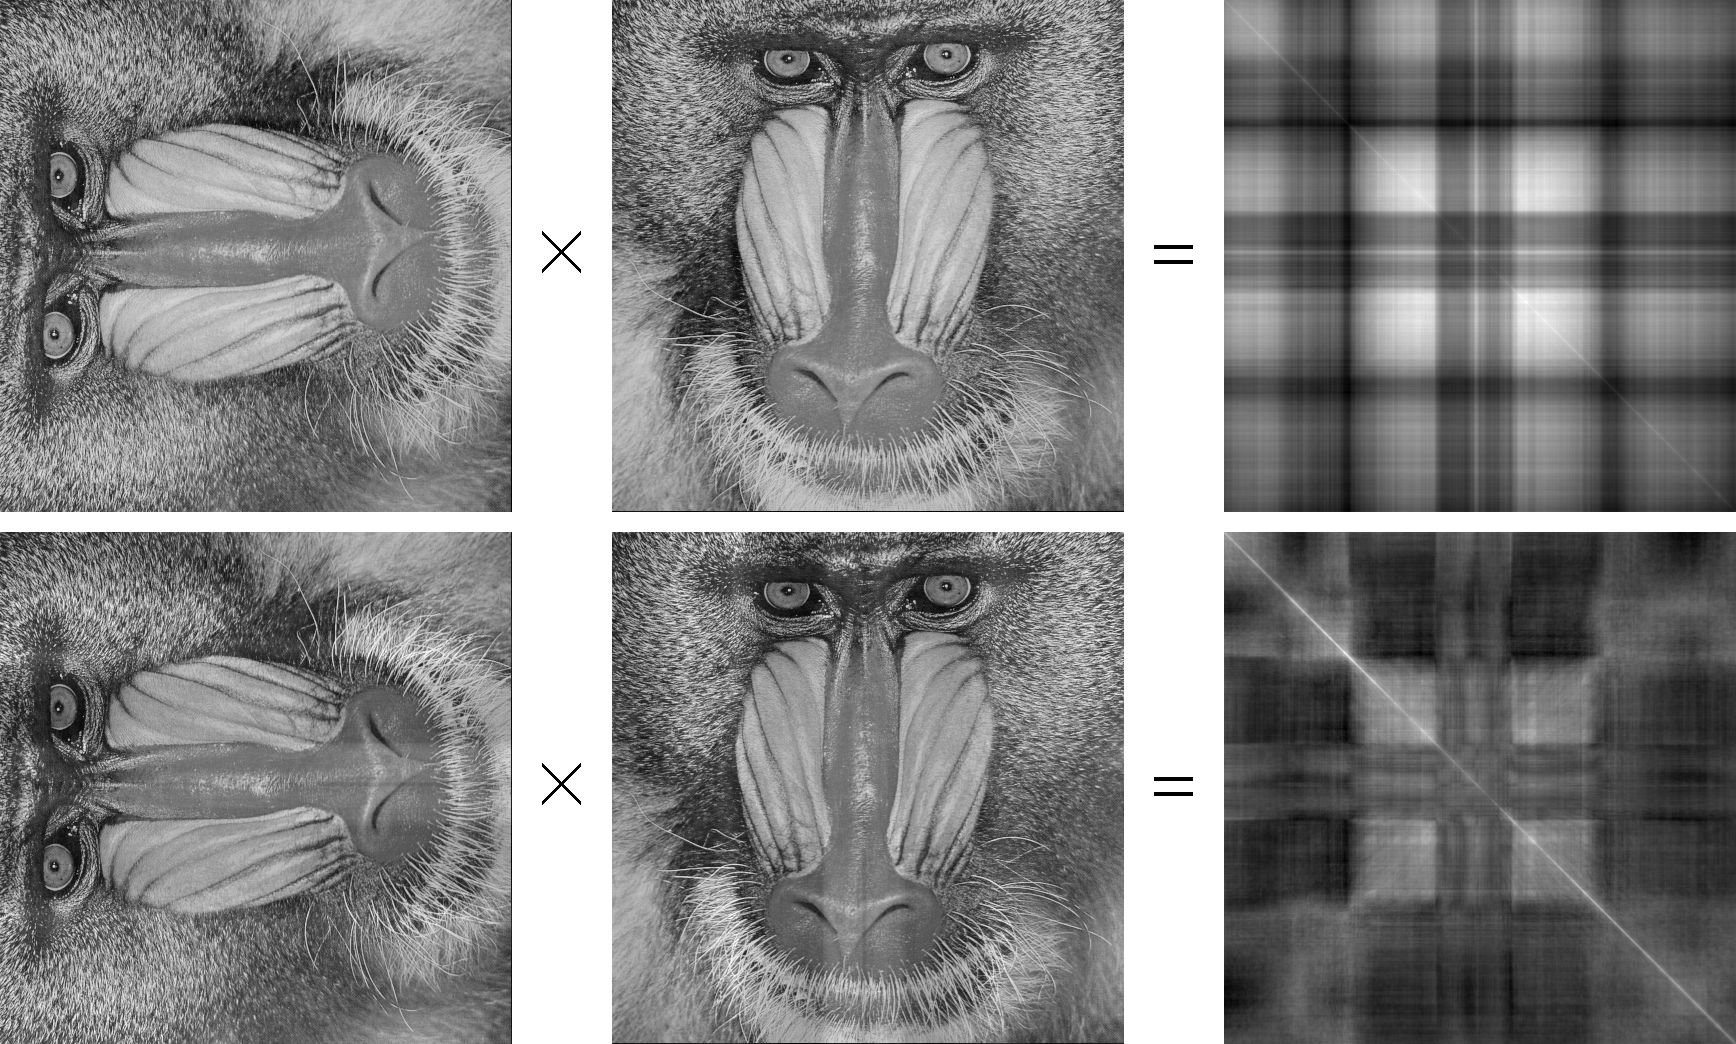
\includegraphics[scale=0.18]{p12}

{\scriptsize In Transformers people sometimes {\bf softmax} rows of the left matrix:\\[-0.1ex]
Attention($Q, K, V$) = softmax($cKQ^T$)$V$ from ``Attention Is All You Need" (2017).\\[-0.5ex]
In the second example we {\bf softmax} rows of the left matrix {\bf and} columns of the right}\\[-0.8ex]
{\scriptsize matrix resulting in products with richer, more fine-grained structure.}


\end{frame}

\begin{frame}

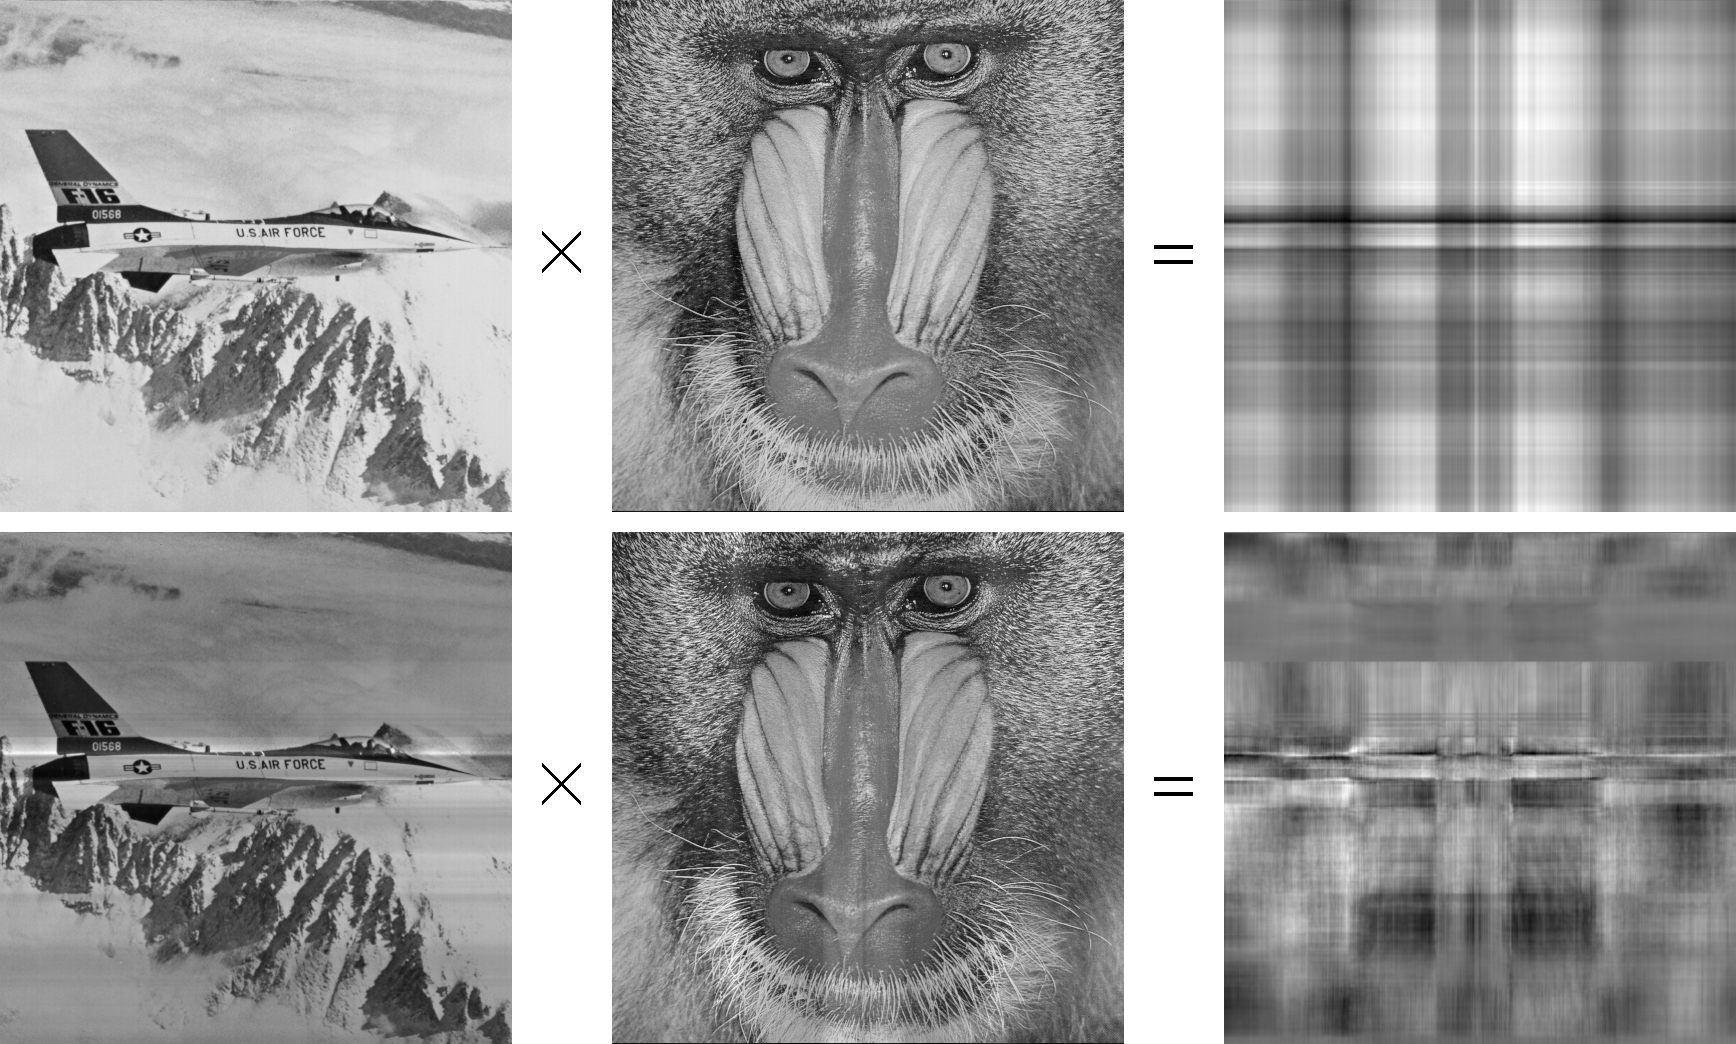
\includegraphics[scale=0.18]{p34}

{\scriptsize In Transformers people sometimes {\bf softmax} rows of the left matrix:\\[-0.1ex]
Attention($Q, K, V$) = softmax($cKQ^T$)$V$ from ``Attention Is All You Need" (2017).\\[-0.5ex]
In the second example we {\bf softmax} rows of the left matrix {\bf and} columns of the right}\\[-0.8ex]
{\scriptsize matrix resulting in products with richer, more fine-grained structure.}

\end{frame}

\begin{frame}

\frametitle{Visual synthesis in the style of digital audio synthesis}

Digital audio synthesis has been almost always done via {\bf composition of unit generators}.\\[2ex]

This style was invented by Max Mathews at Bell Labs in 1957.\\[2ex]

\href{https://en.wikipedia.org/wiki/Max\_Mathews}{\tt\small https://en.wikipedia.org/wiki/Max\_Mathews}\\[2ex]

One should think about those compositions of unit generators as \msmagenta{handcrafted, hand-tuned custom
neural machines}.\\[2ex]

E.g. a typical neuron might have this activation function: $f(a,b,x) = \sin (a*x+b)$.\\[2ex]

Here we are talking about synthesis of images and animations in the same style, but with
{\bf high-dimensional flows} instead of\\ flows of numbers.

\end{frame}

\begin{frame}

  \frametitle{Contact info}

Contact: \href{https://github.com/anhinga}{\tt\small github:anhinga} (e.g. open an issue)\\[2ex]

bukatin@cs.brandeis.edu (or michael.bukatin at gmail)\\[2ex]

\hspace{2.1in}\msmagenta{I am looking for collaborations}  

\end{frame}

\end{document}
